\chapter{Justifications des choix}

\section{Réservoir pour les billes mixtes}

\subsection{Dimensionnement}
Les parois du réservoir initial mesurent \SI{15}{\milli\metre} de hauteur: elles permettent d'éviter que des billes ne soient perdues si elles sont versées avec soin, tout en économisant de la matière par rapport à des parois sur-dimensionnées. 
Ensuite, la pente de \ang{3} du fond du réservoir assure la descente des billes vers le distributeur, mais avec une vitesse modérée. De plus, les interactions des billes entre elles renforcent ce phénomène de ralentissement.
Finalement, nous avons calculé la surface du réservoir comme suit:

\[S = L \cdot l = \SI{98}{\milli\metre} \cdot \SI{165}{\milli\metre} = \SI{16170}{\milli\metre\squared}\]

Où $L$ est la longueur du fond du réservoir, et $l$ la largeur.
Ainsi, dans le pire des cas, soit \num{300} billes de \SI{7}{\milli\metre} de diamètre, ces dernières peuvent se répartir sur l'ensemble du fond du réservoir sans se superposer, si elles sont versées avec soin. En effet, la surface de répartition est donnée par:

\[S\textsubscript{max} = \pi \cdot (\SI{3.5}{\milli\metre})^{2} \cdot \num{300} \cdot \frac{1}{d} \approx  \pi \cdot {\num{3.5}}^{2} \cdot 300 \cdot \frac{1}{0.907} = \SI{12730}{\milli\metre\squared}\]

Où \(d = \frac{ \pi }{2\sqrt{3}} \approx \num{0.907}\) est la densité surfacique de l'arrangement compact de billes.
Cela permet déjà de réduire le risque de problèmes au niveau du distributeur, même si d'autres précautions ont été prises plus loin pour exclure tout coincement.

\subsection{Assemblage}
Pour assembler le fond du réservoir avec les parois, nous avons choisi d'utiliser des goupilles, car des vis aurait exigé un perçage chanfreiné des parois du réservoir pour fixer une vis à tête conique, mais l'épaisseur de \SI{6}{\mm} ne permet pas: cela aurait affaibli le montage, et la tête de la vis aurait dépassé sous la paroi du bord du réservoir. A l'opposé, les goupilles peuvent être fixées grâce à un simple perçage, ce qui renforce l'assemblage.

\section{Acheminement}
\subsection{Choix final}
Après l'évaluation de toutes les options notre choix fut le suivant:
\begin{itemize}
	\item \num{12} cylindres perforés de diamètre \SI{60}{\milli\metre} et épaisseur \SI{8}{\milli\metre} avec \num{10} trous arrondis de profondeur \SI{5.586}{\milli\metre} (mesuré contre le rayon du cylindre) montés sur une barre.
	\item Deux roulements à bille du type \texttt{S686ZZ} dans lesquelles le distributeur (arbre et les \num{12} cylindres perforés) est fixé.
	\item Une arbre de diamètre \SI{8}{\milli\metre} avec un collet (diamètre \SI{6}{\milli\metre}) aux deux extrémités pour la fixer dans deux roulements à billes. À l'extrémité droite se trouve un filetage (M6) pour fixer la manivelle.
	\item Deux grandes fixations quasi-symétrique des deux cotés. Elle contiennent un évidement pour serrer les roulements à billes, des extrusions avec des taraudages pour fixer le couvercle et deux extrusions pour fixer le réservoir mixte et les rails. La seule différence entre la fixation du côté gauche et celle du côté droit est qu'à droite, au centre de l'évidement, se trouve un alésage traversant pour pouvoir visser la fixation de la manivelle à la barre.
	\item Une manivelle préfabriquée de type disque avec un taraudage (M6) pour la fixer. Le disque a un diamètre de \SI{80}{\milli\metre} et un rayon de rotation  \SI{32}{\milli\metre}.
	\item Un couvercle empêchant que les billes ne tombent dans les derniers \ang{45} de l'acheminement à partir de l'horizontale.
\end{itemize}


\subsubsection{Vitesse de tri}
La ligne de contact entre les cylindres perforés et le réservoir est de \SI{96}{\milli\metre}. Le diamètre moyen d'une bille est \SI{6}{\milli\metre}. Sur la ligne de contact se trouveront alors

\[\frac{\SI{96}{\milli\metre}}{\SI{6}{\milli\metre}} = \num{16}\]
billes. À la surface de contact, il y a \num{8} trous à la fois à disposition qui seront donc tous remplis. De plus, lorsque la manivelle fait un tour entier, on pourra potentiellement acheminer 
\[N = (\text{nombre de trous par cylindre}) \cdot (\text{nombre de cylindres}) = \num{10} \cdot \num{12} = \num{120}\]
billes.
On considère que jusqu'à ce qu'il ne reste plus que \num{50} billes dans le réservoir, la surface de contact sera remplie entièrement (pour avoir encore plus de certitude, nous calculerons avec une marge de sécurité de \num{0.9}).
Ainsi, si on commence dans une position de départ où les billes peuvent directement entrer et qu'on achemine \num{120} billes par tour, on va acheminer \num{250} billes en \SI{2.315}{\s} avec une vitesse de rotation $\omega$ d'un tour par seconde.

\[\frac{\theta}{\omega} = \frac{\frac{250 \cdot 2\pi}{120 \cdot 0.9}}{\frac{2\pi}{s}} = \frac{250}{108} \ s = \SI{2.315}{\s}\]

où $\theta$ est l'angle à parcourir pour acheminer 250 billes.

Les \num{50} dernières billes vont s'acheminer un peu plus lentement, vu que la probabilité qu'elles tombent directement sur un trou diminue. Au lieu de faire un calcul exponentiel très compliqué, partons de l'approximation qu'elles soient entraînées avec une certitude de \SI{50}{\percent}. Ce qui fait que

\[\frac{\theta}{\omega} = \frac{\frac{(50 \cdot 2)\pi}{120 \cdot 0.5}}{\frac{2 \pi}{s}} = \frac{50}{60} \ s = \SI{0.833}{\s}\]

\num{0.833} secondes supplémentaires suffiront.
En un total de \SI{3.148}{\sec}, toutes les billes auront alors passé le mécanisme d'acheminement.


\subsection{Acheminement}
La première question qui se pose est de savoir si les billes de diamètre \SI{5}{\mm} vont rester dans leurs cases pendant les premiers \ang{150} de leur tour (cf. l'angle $\theta$ dans la figure en dessous). En effet, si la condition centripète n'est pas remplie constamment, la force centrifuge (dans le repère tournant) dirigerait les petites billes vers les arrêtes des dents. Il y aura donc un contact qui créerait une perte par résistance au roulement (vu que c'est des billes de roulement, on va considérer qu'elles vont rouler sans glissement) et/ou de la friction. 

\begin{figure}
    \centering
    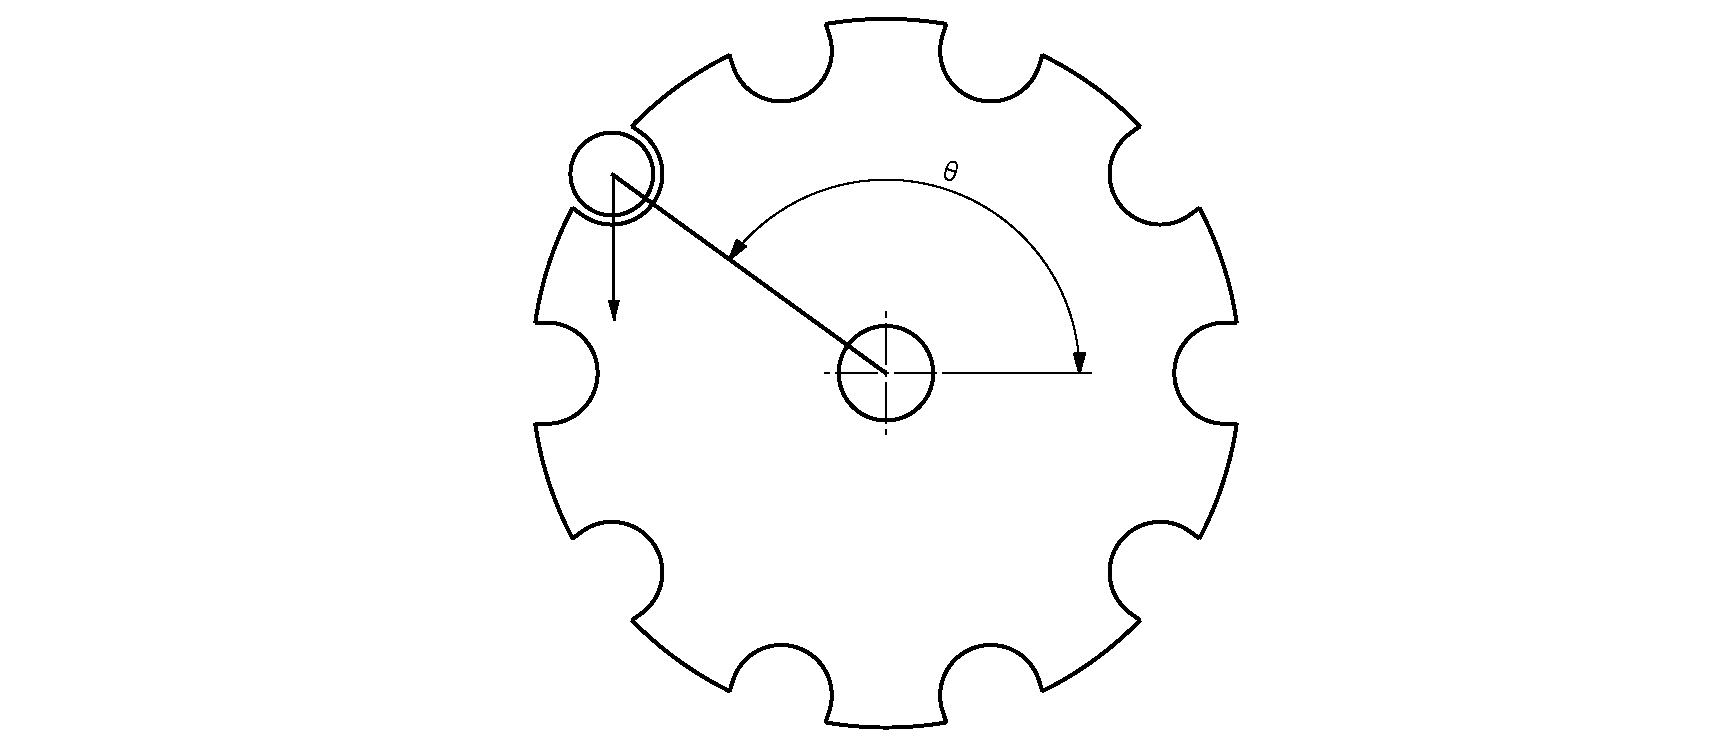
\includegraphics[width=\textwidth]{Graphics/Dessins_justification_Leon/JUST_ANGLE_FAUSSE_COTE.pdf}
    \caption{Angle $\theta$}
    \label{fig:4.1}
\end{figure}

Si nous considérons la figure \ref{fig:4.1}, l'accélération centripète est donnée par:
\[ma_{c} = mg \cdot \sin{\theta}\]

Pour une vitesse de rotation de \(\frac{2 \pi}{s}\), la condition centripète reste remplie pour tout angle supérieur à 

\[\cancel{m} \cdot g \sin{\theta} = \cancel{m} \frac{v^{2}}{R + r} = \cancel{m} \cdot \omega^{2} \ (R +r)\]

\[\sin{\theta} = \frac{\omega^{2} \ (R + r)}{g} = \frac{\frac{4 \pi^{2}}{s^{2}}\ (\SI{24.414}{\milli\metre} + \SI{2.5}{\milli\metre})}{\SI{10}{\m\per\s\squared}} = \frac{\frac{4 \pi^{2}}{s^{2}} \ (\SI{26.914}{\milli\metre})}{\SI{10}{\m\per\s\squared}} \approx 0.0388\]

\[\theta = \arcsin(0.0338) \approx \ang{2.224}\]

Il reste à faire des calculs pour deux cas particuliers. Est-ce que le centre de masse de la bille entrera en contact avec le couvercle entre \(\theta = \ang{2.224}\) et \(\theta = \ang{0}\)? Et comment vont se comporter les billes dans les derniers \ang{60} de la rotation (entre \(\theta = \ang{0}\) et \(\theta = \ang{-60}\)).

\subsubsection{Premier cas ($\theta = \ang{2.224}$ jusqu'à $\theta = \ang{0}$)}

Vu que dans cette partie de la rotation la condition centripète n'est plus satisfaite, la bille va commencer à rouler hors de son logement. Pour faciliter les calculs, considérons que la bille soit un point matériel qui se déplace sans friction en direction du couvercle entre $\theta = \ang{2.224}$ et $\theta = 0$. 
Cette approximation assez forte est tout à fait valable. En effet, si l'on calcule l'accélération de la bille sans prendre en compte la friction, la résistance au roulement et l'énergie convertie en énergie de rotation, je majore celle-ci. C'est-à-dire que si la bille n'entre pas en contact avec le couvercle dans le calcul approximé, elle ne le fera sûrement pas en réalité.\\

On a alors l'équation suivante pour la deuxième loi de Newton (dans le repère tournant):
\[ma = m \frac{\omega^{2}}{(R + r)}\]

\[a = \omega \ (R + r) = \frac{4 \pi^{2}}{s^{2}} \ (\SI{26.914}{\milli\metre}) = 1.063 \ \frac{m}{s^{2}}\]

Le déplacement $\Delta\theta$ entre $\theta =\ang{2.224}$ et $\theta = 0$ va prendre
\[2 \pi \estimates \SI{1}{\s}\]
\[0.0185 \estimates t \]
\[\rightarrow t = \SI{1}{\s} \frac{0.0185}{2 \pi} = \SI{0.00294}{\second}\]

et donc la bille se déplacera de 

\[s = \frac{1}{2} \ a \ t^{2} = \frac{1}{2} \ 1.063 \ \frac{m}{s^{2}} \ (\SI{0.00294}{\s})^{2} = \SI{0.00459}{\milli\metre}\]

Ceci est inférieur à la distance 
\[d = b - 2r = \SI{8.086}{\milli\metre} - 2 \cdot \SI{2.5}{\milli\metre} = \SI{3.086}{\milli\metre}\]

où $b$ est la distance entre le fond et le couvercle et on en soustrait $2r$, car le centre de masse se trouve à distance $r$ du fond et la bille n'a justement pas le droit de se trouver qu'à distance $r$ du couvercle (car dans ce cas la il y aura du contact.

\subsubsection{Deuxième cas ($\theta = \ang{0}$ jusqu'à $\theta = \ang{-60}$)}
Dans les derniers \ang{60}, la condition centripète ne sera plus satisfaite. Ceci va créer un contact avec l'intérieur de la perforation et avec le couvercle. Mais vu que même pour les billes de rayon \SI{5}{\milli\metre}, le centre de masse ne pourra pas dépasser le rayon rouge (\ref{fig:4.2}), cela ne bloquera pas le mécanisme.

\begin{figure}
    \centering
    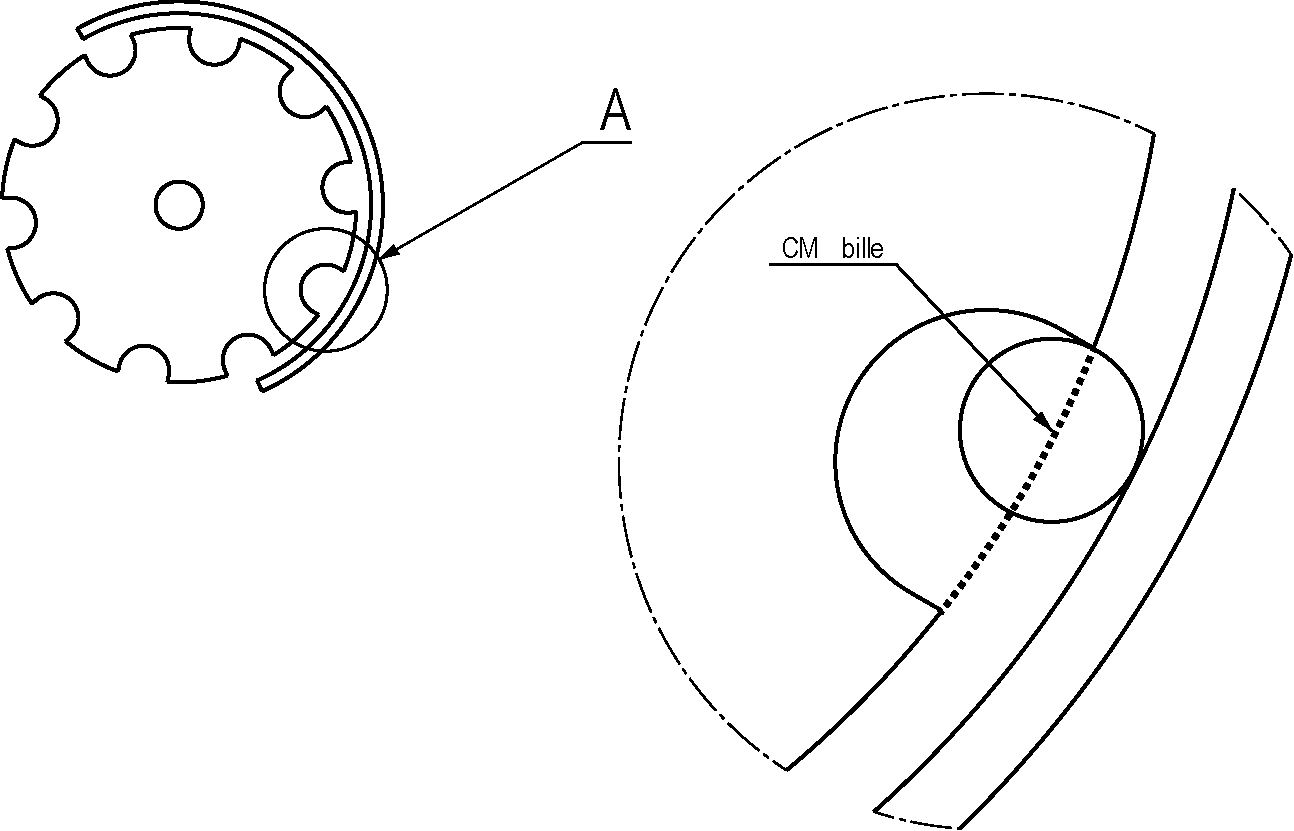
\includegraphics[width=\textwidth]{Graphics/Dessins_justification_Leon/DESSIN_BLOQUAGE_IMPROBLEMATIQUE_FAUSSE_COTE.pdf}
    \caption{Blocage non problématique}
    \label{fig:4.2}
\end{figure}

Par contre, cela créera une perte d'énergie qui sera traité dans le paragraphe suivant.

\subsection{Rendement et sollicitation}
Pour garantir au consommateur une utilisation facile et un fonctionnement durable, il reste à vérifier si notre mécanisme se laisse opérer avec un effort acceptable et s'il y a pas de fortes frictions qui vont créer de l'usure néfaste trop rapidement. L'acheminement fut conçu en minimisant les surfaces de contact avec les éléments statiques afin de minimiser la friction. En considérant \ref{fig:4.3}, on trouve qu'il y a les moments suivants en jeu (vu que les cylindres sont entre eux décalés de \ang{18} chaque deuxième cylindre a ses trous de nouveau au même endroit. Du coup on considère deux cylindres (cf. \ref{fig:4.3}) et multiplie le résultat par 6 pour obtenir ce qu'on a avec \num{12} cylindres.)

\begin{itemize}
    \item La force appliqué par la main qu'on assume perpendiculaire au rayon la manivelle
\[F\textsubscript{main} \cdot r\textsubscript{manivelle}\]

    \item Pour les \num{4} billes dans les derniers \ang{60} la force de friction est \(F\textsubscript{normale}\cdot \mu\) (où $F\textsubscript{normale}$ est égal à $F\textsubscript{centrifuge} $) et celle ci est perpendiculaire à son bras de levier $R\textsubscript{ext}$
\[\frac{1}{2} \; R_{ext} \; \mu \; m\textsubscript{bille} \; \omega^{2} \; R\textsubscript{ext}\]

    \item La force de gravité de toutes les billes fois le bras de levier qui est égal au produit de $R\textsubscript{int}$ et le cosinus de l'angle (moyen) entre la bille et l'horizontale
\[m\textsubscript{bille} \; g\; R\textsubscript{int} \; (\cos(\ang{141.8}) + \cos(\ang{123.8}) + \cos(\ang{105.8}) + \cos(\ang{87.8}) + \cos(\ang{69.8}))\]

\end{itemize}

Pour que notre système soit en équilibre (ou dans notre cas un $\omega$ constant) l'équation suivante (composition des moments d'en haut) s'impose:

\begin{figure}
    \centering
    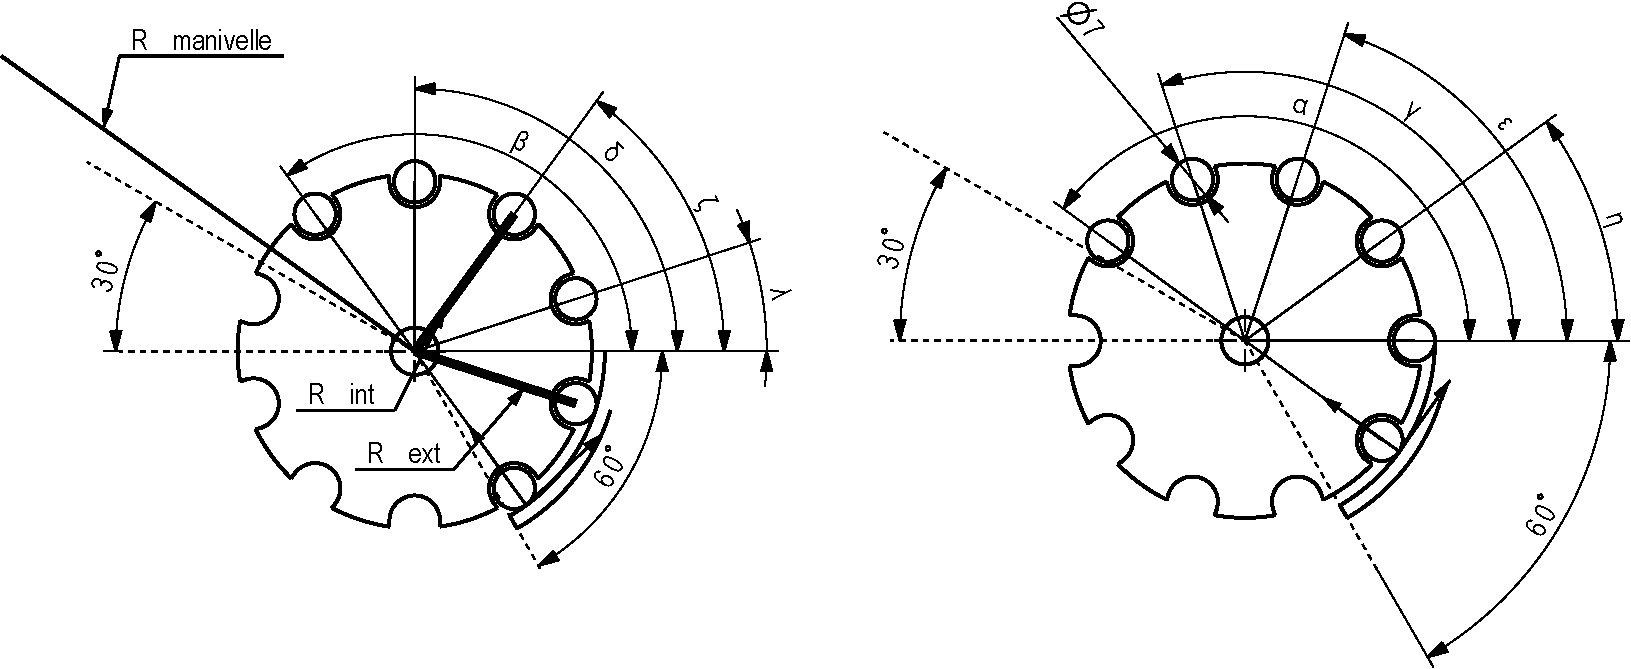
\includegraphics[width=\textwidth]{Graphics/Dessins_justification_Leon/JUST_COS_FAUSSE_COTES.pdf}
    \caption{Angles}
    \label{fig:4.3}
\end{figure}

\[-F\textsubscript{main} \cdot r\textsubscript{manivelle} + \frac{4\cdot 6}{2}\; R\textsubscript{ext}\; \mu \;m\textsubscript{bille} \;\omega^{2}\; R\textsubscript{ext}\]

\[- 8\cdot 6 \ m\textsubscript{bille}\; g\; R\textsubscript{int} \; (\cos(\alpha) + \cos(\beta) + \cos(\gamma \cos(\delta) + \cos(\epsilon)\]

\[- 8\cdot 6 \ m\textsubscript{bille}\; g\; R\textsubscript{int} \; (\cos(\ang{141.8}) + \cos(\ang{123.8}) + \cos(\ang{105.8}) + \cos(\ang{87.8}) + \cos(\ang{69.8})\]

\begin{equation}
    + \cos(\zeta) + \cos(\eta) + \cos(\lambda)) = 0
\label{eq:moments_de_force_en_jeu}
\end{equation}

\begin{equation}
    + \cos(\ang{51.8}) + \cos(\ang{33.8}) + \cos(\ang{15.8})) = 0
\label{eq:moments_de_force_en_jeu}
\end{equation}

où 

\begin{table}[htbp]
    \centering
    \begin{tabular}{|c|c|c|c|c|c|c|c|c|}
        \hline
        Angles & $\alpha$ & $\beta$ & $\gamma$ & $\delta$ & $\epsilon$ & $\zeta$ & $\eta$ & $\lambda$\\
        \hline
        Valeurs & \textbf{\ang{141.8}} & \textbf{\ang{123.8}} & \textbf{\ang{105.8}} & \textbf{\ang{87.8}} & \textbf{\ang{69.8}} & \textbf{\ang{51.8}} & \textbf{\ang{33.8}} & \textbf{\ang{15.8}}\\
        \hline
    \end{tabular}
    \caption{Valeurs de l'angle $\beta$ en dépendance de $s$ et $d$}
    %\label{tab:beta_sphere}
\end{table}

\[R\textsubscript{int} = r\textsubscript{perforation} + r\textsubscript{bille} = \SI{24.414}{\milli\metre} + \SI{3.5}{\milli\metre} = \SI{27.914}{\milli\metre}\]

\[R\textsubscript{ext} = r\textsubscript{couvercle} - r\textsubscript{bille} = \SI{32.5}{\milli\metre} - \SI{3.5}{\milli\metre} = \SI{29}{\milli\metre}\]

\[m\textsubscript{bille} = V \rho\textsubscript{acier} = \frac{4}{3}\pi r^{3} \; \rho\textsubscript{acier} = \frac{4}{3} \pi \;(\SI{3.5}{\milli\metre})^{3} \; \SI{0.0085}{\g\per\mm\cubed} = \SI{1.410}{\g}\]

et

\[\mu = \mu\textsubscript{acier/alu} = \num{0.4}\]

si maintenant on reformule \ref{eq:moments_de_force_en_jeu} selon $F\textsubscript{main}$

\[F\textsubscript{main} = \frac{12 \; R\textsubscript{ext} \; \mu \; m\textsubscript{bille} \; \omega^{2} \; R\textsubscript{ext} - 48 \cdot \num{1.181} \; m\textsubscript{bille} \; g \; R\textsubscript{int}}{r\textsubscript{manivelle}}\]

\[= \frac{12 \cdot \SI{29}{\milli\metre} \cdot \num{0.4} \cdot \SI{1.410}{\g} \; \pi^{2}\SI{4}{\per\s\squared}\; \SI{29}{\milli\metre} - 48 \cdot \num{1.181}\cdot \SI{1.410}{\g} \; \SI{10}{\m\per\s\squared} \; \SI{27.914}{\milli\metre}}{\SI{32}{\milli\metre}}\]

\begin{equation}
    = \SI{-690.21}{\kg\mm\per\s\squared} = \SI{-0.690}{\N}
    \label{eq:F_main}
\end{equation}

Ce calcul est de nouveau une majoration de la situation. Vu qu'il serait hors de nos compétences de calculer la trace exacte que la bille fait pendant les derniers \ang{60}, on l'approxime avec une bille qui est soudée à sa case et glisse sans rouler. Cette bille se trouve dans un repère tournant, du coup la force normale est égale à la force centrifuge. De plus, on part du principe que toutes les cases sont replies avec les billes les plus lourdes et les plus grandes (diamètre \SI{7}{\milli\metre}).

\subsubsection{Rendement}
L'inertie du cylindre rempli avec au maximum $6 \cdot 12$ billes de diamètre \SI{7}{\milli\metre} et donc

    \[I\textsubscript{tot} = I\textsubscript{distributer} + 6\cdot8 \; \left(\frac{2}{5} \; m\textsubscript{bille} \; r\textsubscript{bille}^{2} + m\textsubscript{bille} \; R\textsubscript{int}^2 \right) + 6\cdot4 \; \left(\frac{2}{5} \; m\textsubscript{bille} \; r\textsubscript{bille}^{2} + m\textsubscript{bille} \; R\textsubscript{ext}^2\right)\]
    
    \[= \SI{312300}{\g\mm\squared} + 48\; \left(\frac{2}{5}\ \SI{1.410}{\g}\cdot (\SI{3.5}{\milli\metre})^{2} + \SI{1.410}{\g}\cdot (\SI{27.914}{\milli\metre})^2\right)\]
    
    \[+ 24 \left(\frac{2}{5} \; \SI{1.410}{\g}\cdot (\SI{3.5}{\milli\metre})^2 + \SI{1.410}{\g}\cdot (\SI{29}{\milli\metre})^2\right) = \SI{393992.562}{\g\cdot mm^2}\]
    
\begin{equation}    
    = \SI{0.000394}{\kg\m\squared}
\label{eq:total_inertia}
\end{equation}

Vu que le tri se fait en \SI{3.148}{\s} à un tour par seconde, $F\textsubscript{main}$ parcourt une distance totale de \(t \omega R = \SI{3.148}{\s}\cdot \SI{2\pi}{\per\s} \SI{32}{\milli\metre} = \SI{632.943}{\milli\metre}\). (Malgré le fait que $F\textsubscript{main}$ est négatif dans notre repère, le travail qu'elle effectue est positif, du coup on calcule avec la valeur absolue.)
À l'aide de \ref{eq:total_inertia} on peut alors calculer

\[E\textsubscript{investie} = E\textsubscript{rot} + W\textsubscript{main}\]

\[E\textsubscript{investie} = \frac{1}{2}\;I\textsubscript{tot}\; \omega^{2} + \vert F_{main}\vert \; d = \]

\[\frac{1}{2}\;\SI{0.000394}{\kg\m\squared}\;(\SI{2\pi}{\per\s})^{2} + \SI{0.690}{\N} \cdot \SI{0.632}{\metre} = \SI{0.437}{\J}\]

L'énergie qui ressort est la somme des énergies cinétiques des billes à \ang{-60}

\[E\textsubscript{finale} = \frac{1}{2}\;I\textsubscript{tot}\; \omega^{2} + 300 \cdot \frac{1}{2} \;m\textsubscript{bille}\; \omega^{2} \; R\textsubscript{ext}^{2}\]

\[=\frac{1}{2}\;\SI{0.000394}{\kg\m\squared}(\SI{2\pi}{\per\s})^{2} + 150\; (\SI{2\pi}{\per\s})^{2}\; (\SI{29}{\milli\metre})^2 \cdot \SI{1.410}{\g} =\]
\[\SI{0.00702}{\J}\]

D'où le rendement

\[\eta = \frac{E\textsubscript{finale}}{E\textsubscript{investie}} = \frac{\SI{0.00702}{\J}}{\SI{0.439}{\J}} = \SI{1.6}{\percent} \]

\subsection{Déblocage}
Finalement, il reste à évaluer s'il y a un empilement possible dans les empoches des cylindres. Un tel empilement aurait comme conséquence que les billes soient très proches sur les rails et se freinent les unes les autres, où même bloquent l'acheminement. Par contre le dessin ci-dessus montre clairement que tout empilement à l'endroit de l'acheminement est absolument impossible. Ceci est dû au fait que le centre de masse de la bille en haut est plus à gauche que son point d'appui. Du coup elle va retomber dans le réservoir mixte.
\begin{figure}
    \centering
    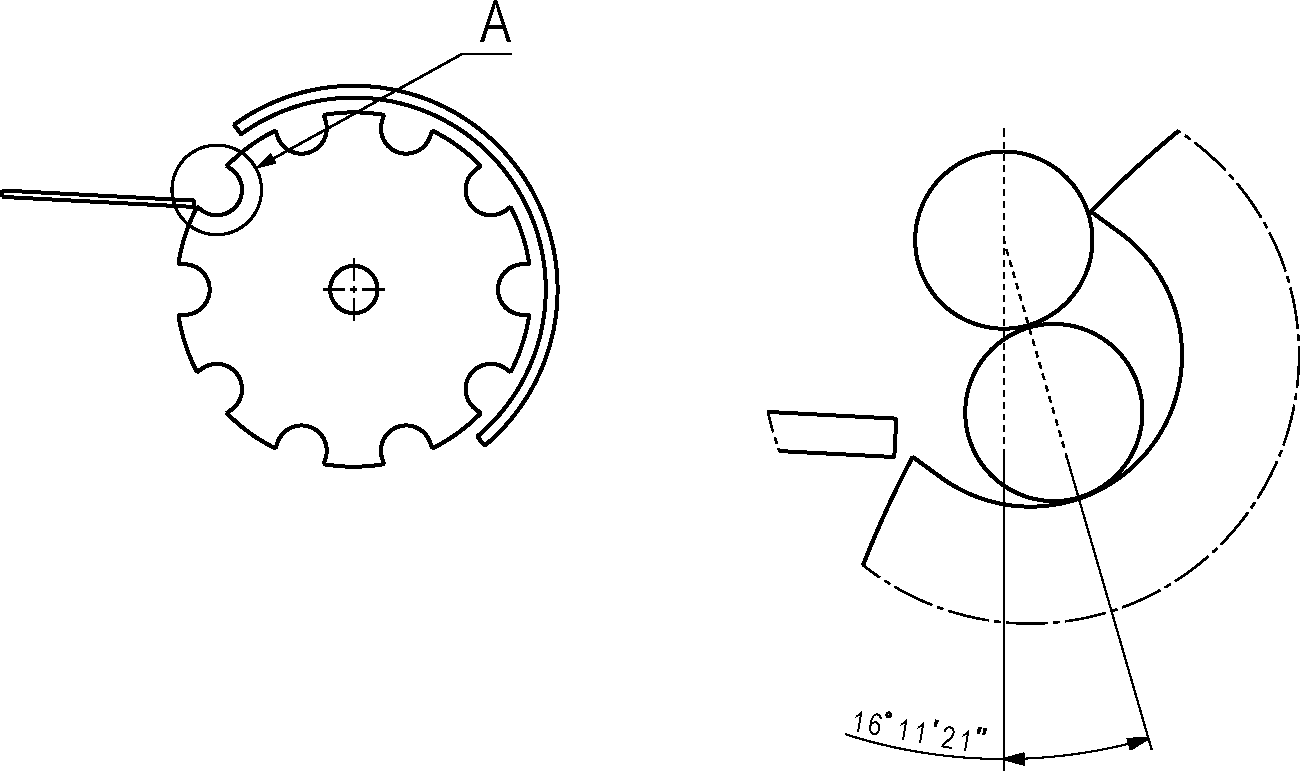
\includegraphics[width=\textwidth]{Graphics/Dessins_justification_Leon/DESSIN_EMPILEMENT_FAUSSE_COTE.pdf}
    \caption{Empilement}
    %\label{fig:B8}
\end{figure}
%dessin manque (DESSIN_EMPILEMENT

\subsection{Sollicitation}
\subsubsection{Flexion de l'arbre}
Pour s'assurer du fait que le matériau de l'arbre soit capable de résister au cisaillement provoqué par l'utilisation il nous faut un petit calcul. De nouveau nous faisons une approximation. On considère que l'arbre est un cylindre sans épaulement qui a un diamètre de \SI{8}{\milli\metre}.
Soient les quantités suivantes:\\
\[r = \SI{4}{\milli\metre} \ (\text{le rayon de l'arbre})\]
\[I_{0} =  (\text{le moment quadratique polaire de la section}) \]
\[M_{t} =  \mit F_{main}\mit \cdot r_{manivelle} = \SI{0.690}{\N}\cdot\SI{32}{\milli\metre} = \SI{22.08}{\N\cdot mm^2} \]
\begin{center}
(le moment de torsion)
\end{center}
\[R_{eg} = \frac{R_{e}}{2} = \frac{\SI{350}{\mega\pascal}}{2} = \SI{175}{\mega\pascal}\]
\begin{center}
(la résistance élastique au cisaillement de l'acier inoxydable)   
\end{center}

Alors on a:
\[\tau_{max} = \frac{M_{t}\cdot r}{I_{0}} = \frac{}{} = ? < R_{eg} = \SI{175}{\mega\pascal}\]
Ceci montre que l'arbre en acier inoxydable réussira à supporter le cisaillement imposé.

\subsubsection{Contrainte sur les roulements}
Les roulements à bille de notre choix \texttt{S686ZZ} sont capables de supporter un poids de \SI{85.3}{\kg} (\SI{853.18}{N}) en dynamique et \SI{34.32}{\kg} (\SI{343.23}{N}) en statique (cf. fichier technique en annexe). L'arbre, les 12 cylindres perforés et la manivelle ensemble pèsent \SI{0.734}{\kg}. Ceci est bien inférieur à \SI{34.32}{\kg}, du coup la durabilité de l'assemblage est assurée.
\section{Séparation et tri}
Pour la séparation et le tri des billes, nous avons choisi la partie avec les rails de tri en avant et les rainures de séparation en arrière, le tout combiné en une seule pièce, appelé le séparateur.

\subsection{Rainures}
Chacune des six rainures amène les billes de deux cylindres sur un seul rail pour le tri. Pour sa forme, nous avons choisi un composé de deux triangles, chaque avec \SI{5,185}{\milli\metre} de haut et \SI{8}{\milli\metre} de large, égale à la largeur d'une roue du distributeur. Ces triangles sont arrangés de manière symétrique de chaque côté de la rainure centrale. Les rainures ne sont pas fraisées perpendiculairement à leur surface normale, mais parallèlement à la pente de la pièce. L'angle d'inclinaison des rainures, dont nous avons besoin pour calculer les points de contact, est donné par:

\[\alpha_{\text{rainure}} = \arctan\left(\frac{\SI{5.185}{\milli\metre}}{\SI{8}{\milli\metre}}\right) \approx \num{0.5751} \approx \ang{32.95}\]

\subsection{Pente}
La pente est donnée par une différence de \SI{2}{\milli\metre} sur la longueur totale de \SI{169}{\milli\metre} de la pièce, donc l'épaisseur projetée de la pièce est de \SI{6}{\mm} au début des rails et de \SI{4}{\mm} à la fin  des rails. Avec les rainures ajoutées, l'épaisseur de la pièce au début est de \SI{9.5}{\mm}. Ces dimensions mènent à une pente de:

\[\alpha_{\text{pente}} = \arctan\left(\frac{\SI{2}{\milli\metre}}{\SI{169}{\milli\metre}}\right) \approx \num{0.0118} \approx \sisetup{add-arc-degree-zero} \ang{;40;}\]

Cette valeur est utilisée pour plusieurs calculs dans la section \ref{calculs_tri}.

\subsection{Ecartement}
\label{ecartements}
L'écartement de la pièce se fait sur deux parties. Dans la première, la distance entre les deux rails est de \SI{5.2}{\mm}, les billes de diamètre \SI{5}{\mm} tombant ainsi dans le réservoir au-dessous, et les plus grandes passent à la prochaine. Dans la deuxième section, la distance entre les deux rails est de \SI{6.2}{\mm}: les billes de diamètre \SI{6}{\mm} tombent ainsi à ce moment, et les billes avec $d = \SI{7}{\mm}$ continuent à rouler jusqu'au bout de la pièce, où elles tombent automatiquement dans le dernier réservoir.

Pour éviter les chocs entre les billes, la transition entre deux écartements différents se fait avec un chanfrein sur une distance de \SI{2}{\mm}. Le même usinage se trouve aussi à la liaison entre les rainures et les rails, et au bout des rails.

Le problème avec un écartement graduel comme démontré dans \ref{ec_graduel}, sera que les billes perdent beaucoup de leur vitesse en avançant sur les rails, ce qui mène à des bouchons et finalement au blocage du mécanisme. Cette relation est donné par \(v = r\omega\) où $v$ est la vitesse linéaire d'une bille, $r$ le rayon de roulement (distance entre point de contact et axe de rotation) et $\omega$ la vitesse angulaire. Comme $r \to 0$ jus qu'avant bille tombe, $v$ va aussi vers 0.

\subsection{Calculs}
\label{calculs_tri}
\subsubsection{Points de contact}
Sur les rainures, la distance entre l'axe de rotation des billes et leur points de contact est donnée par la formule \ref{eq:s_rainure}, $d$ étant le diamètre de la bille. Une esquisse avec les différentes valeurs se trouve sur la figure \ref{fig:esq_rainures_1}.

\begin{equation}
    s_{\text{rainure}}(d) = \cos(\alpha_{\text{rainure}}) \cdot \frac{d}{2} = \frac{1}{\sqrt{\left(\frac{\SI{5.185}{\milli\metre}}{\SI{8}{\milli\metre}}\right)^2+1}} \cdot \frac{d}{2}
    \label{eq:s_rainure}
\end{equation}

Sur les rails, la distance entre l'axe de rotation des billes et leur point de contact est donnée par la formule \ref{eq:s_rails}, où $b$ est la distance entre les deux rails et $d$ le diamètre de la bille. Une esquisse avec les différentes valeurs se trouve sur la figure \ref{fig:esq_rails_1}.

%\[s_{\text{rail}}(d) = 1 - \cos^2\left(\arctan\left(\frac{d}{2}\right)\right)\]

\begin{equation}
    s_{\text{rail}}(d,b) = \sin\left(\arccos\left(\frac{b}{d}\right)\right) \cdot \frac{d}{2} = \sqrt{1-\left(\frac{b}{d}\right)^{2}} \cdot \frac{d}{2}
    \label{eq:s_rails}
\end{equation}

\begin{figure}
    \centering
    \begin{minipage}[c]{0.45\linewidth}
        \centerfloat
        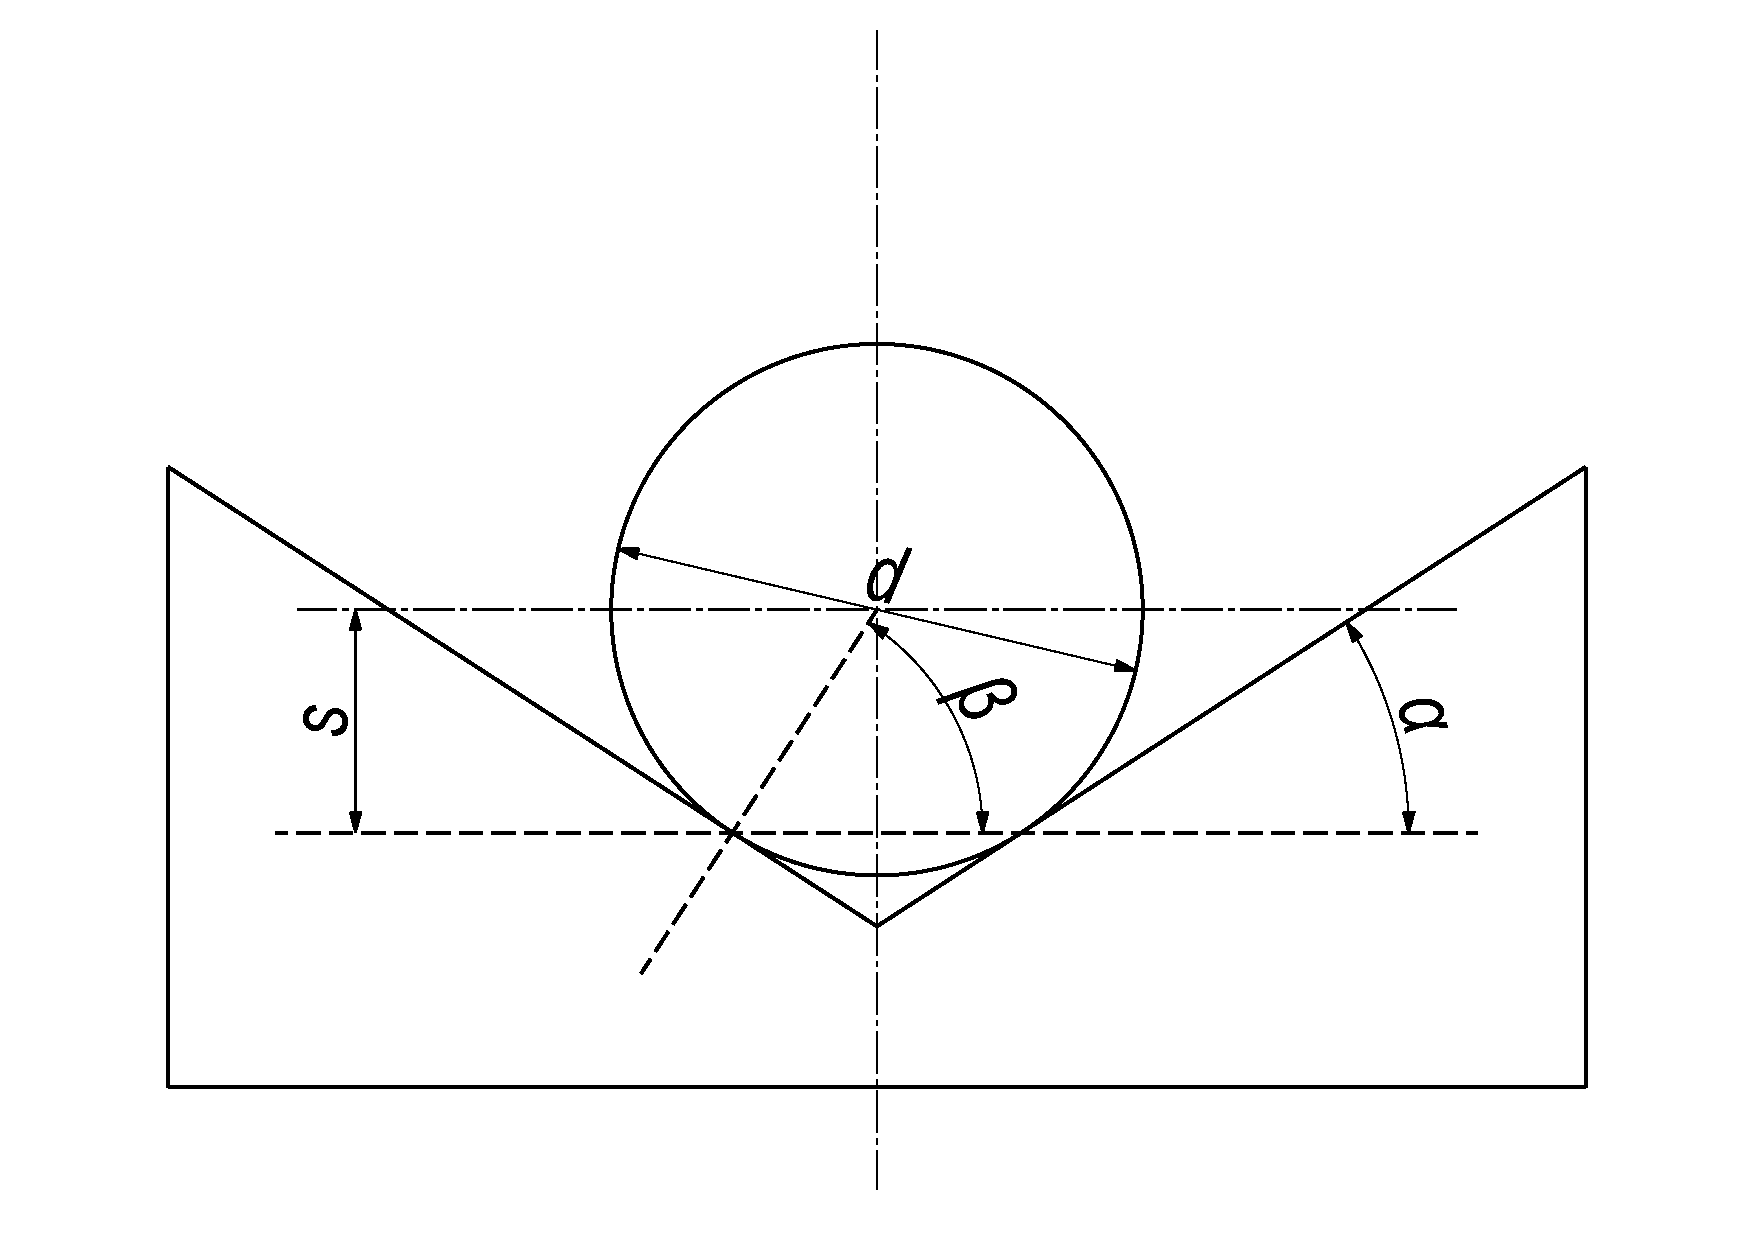
\includegraphics[width=1.25\linewidth]{Graphics/Rails/E_1}
        \caption{Les différentes grandeurs sur une rainure}
        \label{fig:esq_rainures_1}
    \end{minipage}
    \hfill
    \begin{minipage}[c]{0.45\linewidth}
        \centerfloat
        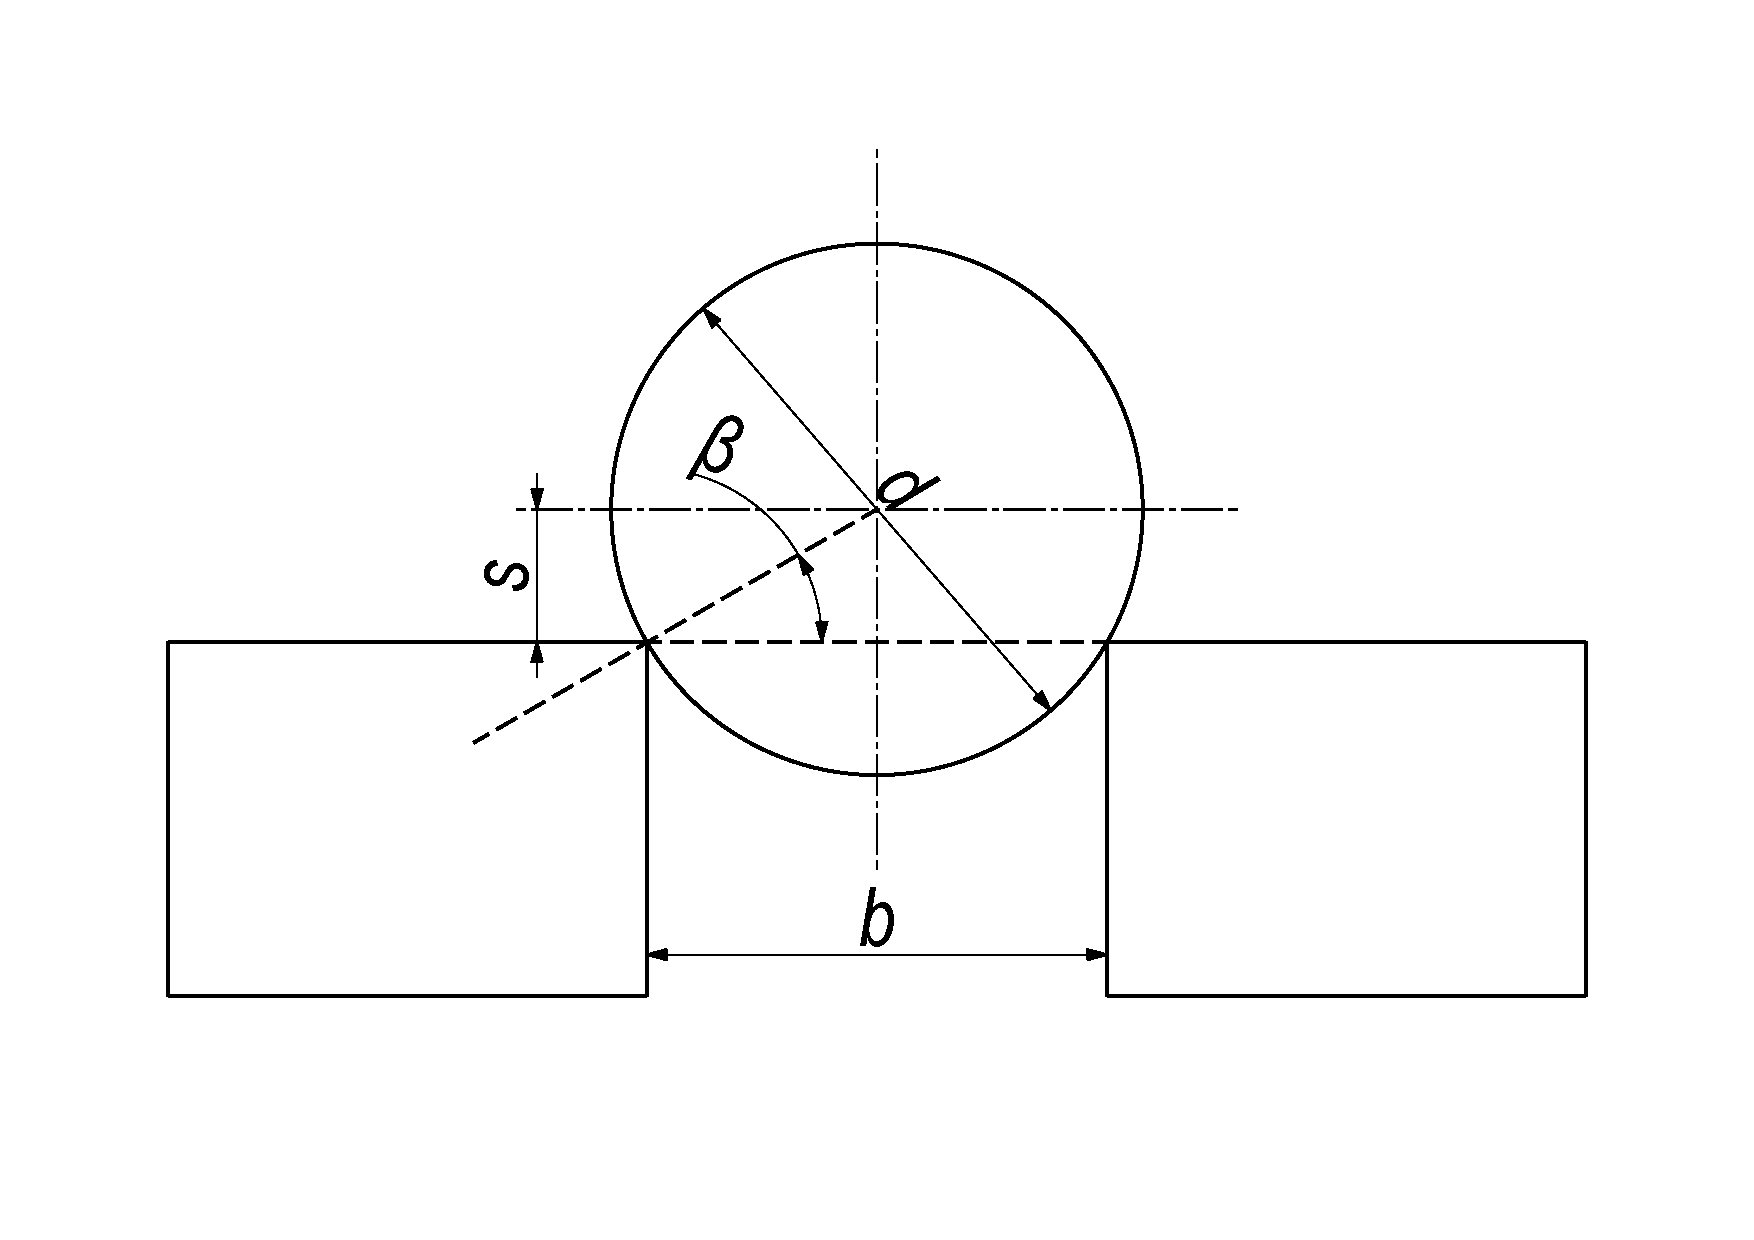
\includegraphics[width=1.25\linewidth]{Graphics/Rails/E_2}
        \caption{Les différentes grandeurs sur un rail}
        \label{fig:esq_rails_1}
    \end{minipage}
\end{figure}

\begin{table}[htbp]
    \centering
    \begin{tabular}{|c|c|c|c|}
        \hline
        Diamètre    & \SI{7}{\mm} & \SI{6}{\mm} & \SI{5}{\mm} \\
        \hline
        Distance    & \textbf{\SI{2.94}{\mm}} & \textbf{\SI{2.52}{\mm}} & \textbf{\SI{2.10}{\mm}} \\
        \hline
    \end{tabular}
    \caption{Valeurs calculés pour la distance verticale entre l'axe de rotation et les points de contact sur les rainures}
    \label{tab:distance_rainures}
\end{table}

\begin{table}[htbp]
    \centering
    \begin{tabular}{|c|c|c|c|}
        \hline
         & \SI{7}{\mm} & \SI{6}{\mm} & \SI{5}{\mm} \\
        \hline
        Rail \SI{5.2}{\mm}& \textbf{\SI{2.34}{\mm}} & \textbf{\SI{1.50}{\mm}} & - \\
        \hline
        Rail \SI{6.2}{\mm}& \textbf{\SI{1.62}{\mm}} & - & - \\
        \hline
    \end{tabular}
    \caption{Valeurs calculées pour la distance verticale entre l'axe de rotation et les points de contact sur les rails. Les billes de diamètre \SI{5}{\mm} n'ont pas de valeurs, car elles tombent directement et ne roulent jamais sur les rails.}
    \label{tab:distance_rails}
\end{table}

\subsubsection{Condition de roulement sans glissement}
La condition pour que les billes roulent sur les rails sans glissement est donnée par la formule \ref{eq:rolling_condition}.

\begin{equation}
    \tan(\alpha_{\text{pente}}) < \mu \frac{7}{2\sin{\beta}}
    \label{eq:rolling_condition}
\end{equation}

\[\beta(d,s) = \arcsin\left(\frac{s}{d/2}\right)\]

%= \arcsin\left(\frac{\SI{1.62}{\milli\metre}}{\SI{7}{\milli\metre}/2}\right)
%  \approx \num{0.2335} \approx \ang{13.381}
%gegenkathete / hypotenuse = sin

\begin{itemize}[label={}, noitemsep]
	\item $\alpha_{\text{pente}}$ \tabto{\tabtoX} Angle d'inclinaison de la pente
	\item $\beta$ \tabto{\tabtoX} Angle de la force normale de la bille au point de contact
	\item $\mu$ \tabto{\tabtoX} Coefficient de frottement entre les rails et les billes
	\item $s$ \tabto{\tabtoX} Distance entre l'axe de rotation et les points de contact
\end{itemize}

En insérant les différentes valeurs pour $s$ et les diamètres $d$ correspondants, on obtient les valeurs notées dans le tableau \ref{tab:beta_sphere}.

\begin{table}[htbp]
    \centering
    \begin{tabular}{|c|c|c|c|}
        \hline
         & \SI{7}{\mm} & \SI{6}{\mm} & \SI{5}{\mm} \\
        \hline
        Rainures & \textbf{\ang{57.05}} & \textbf{\ang{57.05}} & \textbf{\ang{57.05}} \\
        \hline
        Rail \SI{5.2}{\mm}& \textbf{\ang{42.02}} & \textbf{\ang{29.93}} & - \\
        \hline
        Rail \SI{6.2}{\mm}& \textbf{\ang{27.66}} & - & - \\
        \hline
    \end{tabular}
    \caption{Valeurs de l'angle $\beta$ en dépendance de $s$ et $d$}
    \label{tab:beta_sphere}
\end{table}

Pour confirmer le fait que les billes roulent sans glissement sur toute la longueur de la pièce de séparation de tri, la valeur du plus petit angle $\beta$ du tableau \ref{tab:beta_sphere} est insérée dans la formule \ref{eq:rolling_condition}. Ceci est l'angle de la bille de $d = \SI{7}{\mm}$ sur le rail avec écartement $s = \SI{6.2}{\mm}$. $\mu$ a la même valeur que précédemment, égal à \num{0.4}.

\[\sisetup{add-arc-degree-zero} \tan(\ang{;40;}) < \num{0.4} \cdot \frac{7}{2\sin(\ang{27.66})}\]

\[\num{0.0118} < \num{3.0157} \quad \checkmark\]

Avec cette relation, nous arrivons à la conclusion que, si les billes roulent, elles roulent sans glissement.

\subsubsection{Accélération}
La vitesse d'une bille avec deux points de contact, comme nous les avons dans notre mécanisme, est donnée par la formule \ref{eq:acceleration_sphere}. Les symboles sont les mêmes que dans la formule \ref{eq:rolling_condition}, avec $f$, égal à $c_{rr}$, le coefficient de résistance au roulement.

\begin{equation}
    \dot{v} = a = \frac{5\sin^{2}(\beta)}{2+5\sin^{2}(\beta)} g(\sin({\alpha_{\text{pente}}) - f\cos(\alpha_{\text{pente}})})
    \label{eq:acceleration_sphere}
\end{equation}

En insérant les valeurs précédentes, $\beta$, et en plus $f = \num{0.001}$, le coefficient de résistance de roulement d'une bille d'acier sur une plaque d'acier, nous obtenons finalement des valeurs pour les accélérations différentes des billes sur la pièce de séparation et tri. Toutes les accélérations sont notées dans le tableau \ref{tab:accelerations_sphere}.

\begin{table}[htbp]
    \centering
    \begin{tabular}{|c|c|c|c|}
        \hline
         & \SI{7}{\mm} & \SI{6}{\mm} & \SI{5}{\mm} \\
        \hline
        Rainures & \textbf{\SI{0.0678}{\m\per\s\squared}} & \textbf{\SI{0.0678}{\m\per\s\squared}} & \textbf{\SI{0.0678}{\m\per\s\squared}} \\
        \hline
        Rail \SI{5.2}{\mm}& \textbf{\SI{0.0562}{\m\per\s\squared}} & \textbf{\SI{0.0408}{\m\per\s\squared}} & - \\
        \hline
        Rail \SI{6.2}{\mm}& \textbf{\SI{0.0372}{\m\per\s\squared}} & - & - \\
        \hline
    \end{tabular}
    \caption{Valeurs des accélérations ($a$) en dépendance de $\beta$}
    \label{tab:accelerations_sphere}
\end{table}

\subsubsection{Vitesses}

% Par intégration de la formule \ref{eq:acceleration_sphere}, l'équation de vitesse peut être calculée.

% \begin{equation}
%     v = \int \dot{v} \ dt = \frac{-5(\sin({\alpha_{\text{pente}}) - f\cos(\alpha_{\text{pente}})})g \cdot t}{7} + v_{0}
%     \label{eq:velocity_sphere_alg}
% \end{equation}

Pour déterminer les expressions pour la vitesse finale et le temps nécessaire pour traverser la pièce, il faut premièrement calculer la vitesse initiale ($v_{0}$) quand les billes arrivent sur la pièce. La vitesse finale des billes quand elles quittent le distributeur est égale à la vitesse initiale au début du séparateur. Le rayon $r$ est la distance entre le centre de masse de la plus grande bille et l'axe de rotation du convoyeur. En supposant un tour par seconde de la manivelle ($\omega = 2\pi$), $v_{0}$ est calculé comme suit:

\begin{equation}
    v_{0} = \omega r = \SI{2\pi}{\per\second} \cdot \SI{29}{\mm} \approx \SI{182.212}{\mm\per\s} \approx \SI{0.182}{\m\per\s}
    \label{eq:initialV_rails}
\end{equation}

\[r = \SI{32.5}{\mm} - \left(\frac{\SI{7}{\mm}}{2}\right) = \SI{29}{\mm}\]

Avec toutes ces valeurs, nous pouvons finalement calculer les vitesses des billes sur différentes parties de la pièce, quand elles quittent la pièce et tombent dans le réservoir final correspondant, et le temps nécessaire pour chacune de ces valeurs.

Ici, les vitesses sont déterminées à travers les accélérations et les distances. Comme la longueur supplémentaire de la pente est négligeable en comparaison avec la longueur totale de la pièce (voir formule \ref{eq:length_neglect}), tous les calculs sont faits sur la longueur horizontale.

\begin{equation}
    l = \sqrt{\text{hauteur}^2 + \text{longueur}^2} = \sqrt{(\SI{2}{\mm})^2 + (\SI{169}{\mm})^2} \approx \SI{169.012}{\mm} \approx \SI{169}{\mm}
    \label{eq:length_neglect}
\end{equation}

Les billes arrivent sur la pièce à une position $A$, à environ \SI{20}{\mm} du bout de la pièce. Les billes de \SI{5}{\mm} de diamètre roulent sur la distance $\overline{AB}$, les billes de \SI{6}{\mm} sur la distance $\overline{AC}$ et les billes de \SI{7}{\mm} sur la distance $\overline{AD}$. Les distances entre les différents points se trouvent dans la figure \ref{fig:distances_rails} et dans le tableau \ref{tab:sphere_rolling_distance}.

\begin{figure}
    \centering
    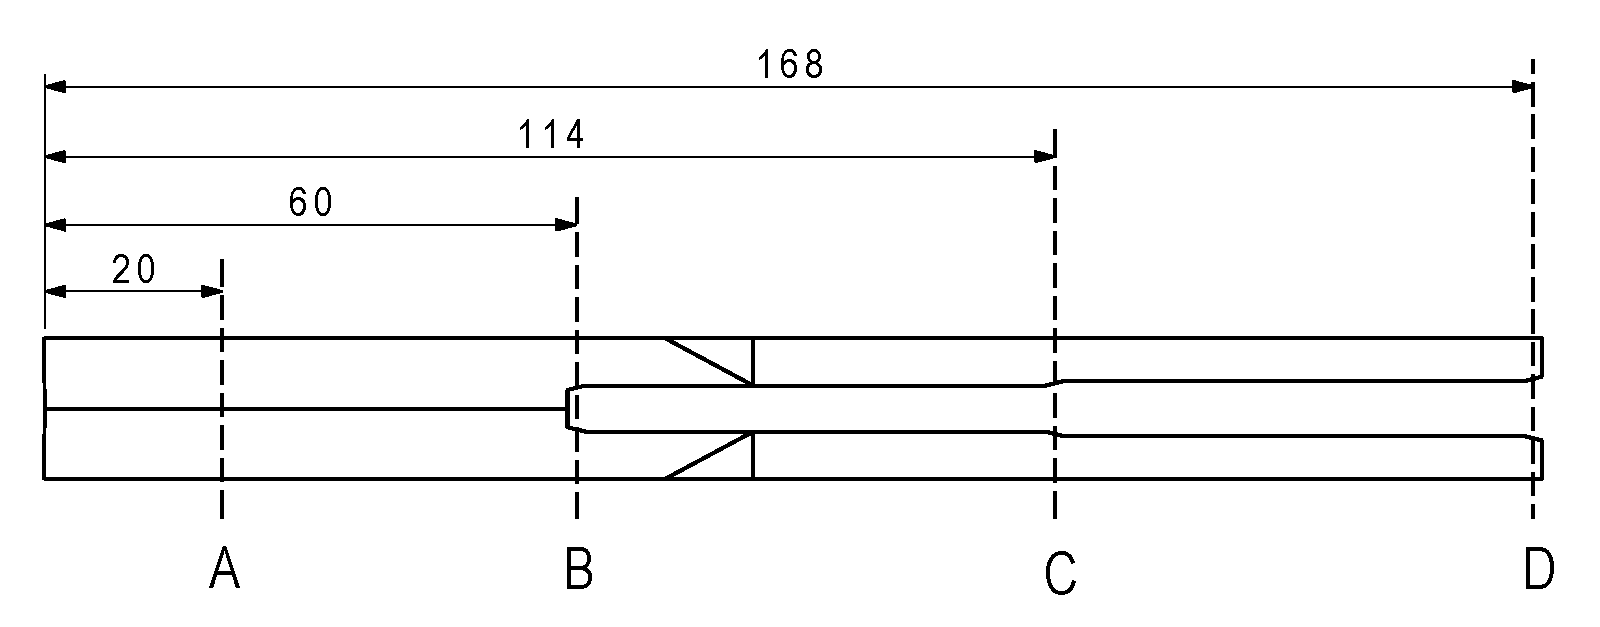
\includegraphics[width=\textwidth]{Graphics/Rails/DISTANCES.pdf}
    \caption{Distances sur un rail}
    \label{fig:distances_rails}
\end{figure}

\begin{table}[htbp]
    \centering
    \begin{tabular}{|c|c|c|c|}
        \hline
        $\overline{AB}$ & $\overline{BC}$ & $\overline{CD}$ & Total \\
        \hline
        \SI{40}{\mm} & \SI{54}{\mm} & \SI{54}{\mm} & \SI{148}{\mm} \\
        \hline
    \end{tabular}
    \caption{Distances parcourues ($d$) par les billes entre différents points sur la pièce}
    \label{tab:sphere_rolling_distance}
\end{table}

Les valeurs trouvées pour les accélérations en \ref{eq:acceleration_sphere}, la vitesse initiale de \ref{eq:initialV_rails} et les distances de \ref{tab:sphere_rolling_distance} sont insérées dans la formule \ref{eq:velocities_spheres} pour obtenir les vitesses finales en calculant les différentes accélérations sur les différentes distances parcourues. Les valeurs en gras représentent les vitesses finales des billes quand elles tombent dans la pièce au-dessous.

\begin{equation}
    v=\sqrt{2ad +{v_{0}}^{2}}
    \label{eq:velocities_spheres}
\end{equation}

\begin{table}[htbp]
    \centering
    \begin{tabular}{|c|c|c|c|}
        \hline
         & \SI{7}{\mm} & \SI{6}{\mm} & \SI{5}{\mm} \\
        \hline
        $A$ & \SI{0.182}{\m\per\s} & \SI{0.182}{\m\per\s} & \SI{0.182}{\m\per\s} \\
        \hline
        $B$ & \SI{0.197}{\m\per\s} & \SI{0.197}{\m\per\s} & \textbf{\SI{0.197}{\m\per\s}} \\
        \hline
        $C$ & \SI{0.211}{\m\per\s} & \textbf{\SI{0.207}{\m\per\s}} & - \\
        \hline
        $D$ & \textbf{\SI{0.221}{\m\per\s}} & - & - \\
        \hline
    \end{tabular}
    \caption{Valeurs des vitesses ($v$) des billes sur différentes parties de la pièce, la vitesse au point $A$ est égale à $v_{0}$}
    \label{tab:sphere_velocities}
\end{table}

Avec les résultats trouvés dans la table \ref{tab:sphere_velocities}, nous constatons que la seule section où un coincement serait possible se trouve sur le rail avec \SI{5.2}{\mm} d'écartement, à cause de deux types de billes se trouvant au même endroit avec des vitesses déviantes. Mais comme les billes de \SI{7}{\mm} sont seulement \SI{1.9}{\percent} plus rapides que les billes de \SI{6}{\mm}, cette différence est négligeable. Le cas où les billes sautent d'un réservoir au prochain peut aussi être exclu, grâce à la vitesse relativement lente des billes, le revêtement des réservoir, et les parois entre deux réservoirs.

\subsubsection{Temps}
Pour conclure les calculs de cette pièce, les temps nécessaires pour la traverser sont calculés. Ceux-ci se calculent en insérant les valeurs du tableau \ref{tab:sphere_rolling_distance}, du tableau \ref{tab:accelerations_sphere} et de la formule \ref{eq:initialV_rails} dans la formule \ref{eq:rolling_time}. Les résultats se trouvent dans le tableau \ref{tab:results_rolling_time}.

\begin{equation}
     t = \frac{v - v_{0}}{a}
     \label{eq:rolling_time}
\end{equation}

\begin{table}[htbp]
    \centering
    \begin{tabular}{|c|c|c|c|}
        \hline
         & \SI{7}{\mm} & \SI{6}{\mm} & \SI{5}{\mm} \\
        \hline
        $A$ & \SI{0}{\s} & \SI{0}{\s} & \SI{0}{\s} \\
        \hline
        $B$ & \SI{0.211}{\s} & \SI{0.211}{\s} & \SI{0.211}{\s} \\
        \hline
        $C$ & \SI{0.265}{\s} & \SI{0.267}{\s} & - \\
        \hline
        $D$ & \SI{0.250}{\s} & - & - \\
        \hline\hline
        $\Sigma$ & \textbf{\SI{0.726}{\s}} & \textbf{\SI{0.478}{\s}} & \textbf{\SI{0.211}{\s}} \\
        \hline
    \end{tabular}
    \caption{Temps nécessaire ($t$) de chaque type de bille pour traverser la pièce jusqu'au point où elle tombe dans le réservoir approprié}
    \label{tab:results_rolling_time}
\end{table}



% La vitesse finale d'une bille au bout de la pièce se calcule en insérant la valeur de la formule \ref{eq:initialV_rails} dans \ref{eq:velocity_sphere_alg}.

% \[v = \int \dot{v} \ dt = \frac{-5(\sin({\alpha_{\text{pente}}) f\cos(\alpha_{\text{pente}})})g \cdot t}{7} + v_{0}\]

% Le temps $t$, dont une bille a besoin pour traverser la pièce est calculée en \ref{eq:rolling_time}. En avant, la distance parcourue de la bille sur la pièce est calculée.

% \[l = \sqrt{\text{hauteur}^2 + \text{longueur}^2} = \sqrt{(\SI{2}{\mm})^2 + (\SI{169}{\mm})^2} \approx \SI{169.012}{\mm}\]

\section{Réservoir pour les billes triées}
La version finale du réservoir pour les billes triées était le troisième brouillon. Au contraire du premier brouillon, la version finale nous permet d'enlever les réservoirs avec les billes triées séparément, et cela sans que la construction des pièces ne soit difficile, ce qui a exclu le deuxième brouillon. Voici ces deux raisons principales en plus de détail:

\subsection{Réservoirs flexibles}
Quelle que soit l'utilisation des billes triées, la flexibilité des réservoirs, qui permettent d'enlever toutes les billes triées de la même taille en même temps, est bien utile lors de l'utilisation future de la machine. Son efficacité en service est donc bien meilleure que si l'on devait enlever toutes les billes à la main d'un réservoir fixe. Le positionnement exact des réservoirs est garanti par une plaque %{insérer lien dessin sol}
qui entoure les pieds de chacun des réservoirs. Le jeu pour enlever les réservoirs est d'un millimètre en haut ainsi qu'en bas. C'est assez grand pour qu'ils ne se coincent pas, et assez petit pour que la distance entre le haut du réservoir et la prochaine pièce soit de \SI{4}{\mm}, ce qui garantit que même les billes les plus petites trouvent leur chemin dans le bon réservoir, une fois tombées à travers les rails.

\subsection{Usinage}
Nous avons décidé d'augmenter le nombre de pièces afin de simplifier leur usinage. Parmi les pièces utilisées, il n'y a aucune pièce qui ne pouvait pas être usiné par des processus courants, certaines même sans assistance par ordinateur. La décomposition en pièces faciles à usiner est un avantage pour la production, mais pas pour l'assemblage de la machine. Si l'on voulait lancer la machine en production en grande série, il faudrait reconsidérer ce choix. En grand nombre, même des pièces plus complexes sont moins chères car les coûts de la configuration de l'usinage peuvent être répartis sur plusieurs pièces et forment donc une plus petite partie du prix de la pièce. Nous avons estimé que pour notre projet, le surcroît des dépenses se compense facilement par l'économie réalisée pendant l'usinage.

En outre, nous avons fait intervenir des parois qu'il est possible d'acheter bon-marché. En découpant une paroi, nous obtenons une pièce qui s'utilise facilement comme partie d'un réservoir. Comme déjà évoqué, nous avons rejeté l'idée d'ajuster la taille de chaque réservoir à la taille des billes correspondantes, pour augmenter la simplicité dans la production. 

\subsection{Dimensionnement}
Le dimensionnement des cubes se déroulait en prise en compte de la taille des billes. Dans le pire des cas, les \num{300} billes sont de la même taille : les réservoirs doivent alors être capables de contenir \num{300} billes de la taille respective. Pour simplifier la construction, les cubes ont tous la même taille sans respecter la taille des billes.
Nous avons calculé le volume des réservoirs comme suit:
\begin{equation}
    V = \frac{4}{3} \pi r^3 \cdot \num{300} \cdot \frac{1}{d} = \frac{4 \pi \cdot (\SI{3.5}{\mm})^3 \cdot \num{300}}{3 d} \approx \SI{71838}{\mm\cubed}
    \label{eq:volumereservoirfin}
\end{equation}

Où \(d = \frac{\pi}{3\sqrt{2}} \approx \num{0.75}\) est la densité volumique de l'empilement compact de billes.
La taille du rayon interne de la paroi se calcule comme suit:

\begin{equation}r\textsubscript{int} \geq \sqrt{\frac{2\ V}{\pi\ l}}=\sqrt{\frac{2 \cdot \SI{71838}{\mm\cubed}}{\pi\ \SI{90}{\mm}}} \approx \SI{22.5}{\mm} \label{eq:rayonreservoirfin}\end{equation}

Avec $V= \SI{71838}{\mm\cubed}$ calculé par la formule \ref{eq:volumereservoirfin} et $l=\SI{90}{\mm}$ la longueur interne adaptée à la largeur des rails. En ajoutant un petit facteur de sécurité si les billes ne s'empilent pas de la manière la plus compacte possible, et en fixant l'épaisseur de la paroi de \SI{2}{\mm}, nous avons obtenu un rayon externe de la paroi de $r\textsubscript{ext}=\SI{27}{\mm}$. Pour que les billes ne fassent pas trop de bruit lors du choc au réservoir, nous avons prévu un revêtement en feutre d'une épaisseur d'un millimètre. Le rayon interne mesure alors \SI{24}{\mm}, ce qui respecte toujours la limite qu'on a calculé par la formule \ref{eq:rayonreservoirfin}.